% !TEX program = xelatex
\documentclass[9pt, aspectratio=169]{beamer}
\usetheme{metropolis}
\usefonttheme{professionalfonts}

% --- Modern Font Setup ---
\usepackage[T1]{fontenc}
\usepackage{FiraSans}  % Modern, elegant sans-serif font family
\usepackage[scaled=0.95]{FiraMono}  % Matching monospace font

% Lighter, more refined font weights
\renewcommand{\seriesdefault}{l}  % Light weight as default
\renewcommand{\bfseries}{\fontseries{sb}\selectfont}  % Semi-bold instead of bold

% Custom font sizing - more refined
\setbeamerfont{title}{size=\Large, series=\fontseries{m}\selectfont}
\setbeamerfont{subtitle}{size=\normalsize, series=\fontseries{l}\selectfont}
\setbeamerfont{author}{size=\small, series=\fontseries{l}\selectfont}
\setbeamerfont{date}{size=\small, series=\fontseries{l}\selectfont}
\setbeamerfont{frametitle}{size=\normalsize, series=\fontseries{m}\selectfont}
\setbeamerfont{framesubtitle}{size=\footnotesize, series=\fontseries{l}\selectfont}
\setbeamerfont{block title}{size=\normalsize, series=\fontseries{m}\selectfont}
\setbeamerfont{block body}{size=\small}
\setbeamerfont{itemize/enumerate body}{size=\small}
\setbeamerfont{itemize/enumerate subbody}{size=\footnotesize}
\setbeamerfont{section in toc}{size=\normalsize, series=\fontseries{m}\selectfont}
\setbeamerfont{section title}{size=\Large, series=\fontseries{m}\selectfont}

% --- Color Definitions ---
% Primary Theme Colors
\definecolor{PrimaryColor}{RGB}{33,52,72}         % Deep navy
\definecolor{SecondaryColor}{RGB}{84,119,146}     % Desaturated blue-gray
\definecolor{AccentColor}{RGB}{100,156,165}       % Soft steel blue
\definecolor{black}{RGB}{0,0,0}
\definecolor{BackgroundColor}{RGB}{245,247,250}   % Very light cool gray/blue-tinted white
\definecolor{TextColor}{RGB}{40,55,70}            % Darker, cool-toned charcoal
\definecolor{LightGray}{RGB}{220,225,230}         % Soft, cool light gray
\definecolor{DarkGray}{RGB}{70,90,105}            % Cool-toned dark gray

% --- Theme Customization ---
\setbeamercolor{background canvas}{bg=BackgroundColor}
\setbeamercolor{normal text}{fg=TextColor}
\setbeamercolor{frametitle}{bg=PrimaryColor, fg=white}
\setbeamercolor{section in toc}{fg=PrimaryColor}
\setbeamercolor{block title}{bg=PrimaryColor!80, fg=white}
\setbeamercolor{block body}{bg=PrimaryColor!10}
\setbeamercolor{alerted text}{fg=AccentColor}
\setbeamercolor{itemize item}{fg=PrimaryColor}
\setbeamercolor{itemize subitem}{fg=SecondaryColor}

% Progress bar
\setbeamercolor{progress bar}{fg=AccentColor, bg=LightGray}

% --- Packages ---
\usepackage[utf8]{inputenc}
\usepackage{url}
\usepackage{booktabs}
\usepackage{amsmath, amssymb, amsfonts}
\usepackage{fontawesome5}
\usepackage{pifont}
\usepackage[most]{tcolorbox}
\tcbuselibrary{skins, listings}
\usepackage{colortbl}
\usepackage{array}
\usepackage{adjustbox}
\usepackage{ragged2e}

% --- Packages for plotting discrete and continuous signals and spectrums ---
\usepackage{tikz}
\usepackage{circuitikz} % Useful for signal processing block diagrams
\usepackage{pgfplots}
\usepackage{graphicx}
\usepackage{caption}
\usepackage{subcaption}

\usetikzlibrary{shapes.callouts, positioning, arrows.meta, shapes.geometric, shadows, calc, patterns, backgrounds, shadings, fit, chains, decorations.pathreplacing, intersections}
\usepgfplotslibrary{fillbetween}
\usepgfplotslibrary{polar}
\pgfplotsset{compat=1.18}
\pgfplotsset{
    plot coordinates/math parser=false,
    signal/.style={thick, color=PrimaryColor},
    spectrum/.style={thick, color=AccentColor},
    discrete/.style={ycomb, mark=*, mark options={fill=white, draw=PrimaryColor}, color=PrimaryColor, thick},
}

% --- Custom Commands ---
\newcommand{\cmark}{\textcolor{PrimaryColor}{\ding{51}}}
\newcommand{\xmark}{\textcolor{AccentColor}{\ding{55}}}
\newcommand{\highlight}[1]{\textcolor{PrimaryColor}{\textbf{#1}}}

% --- Custom tcolorbox environments ---
\newtcolorbox{conceptbox}[1]{
    colback=PrimaryColor!10,
    colframe=PrimaryColor,
    title=#1,
    fonttitle=\small\bfseries,
    fontupper=\small,
    rounded corners
}

\newtcolorbox{insightbox}[1]{
    colback=AccentColor!10,
    colframe=AccentColor,
    title=#1,
    fonttitle=\small\bfseries,
    fontupper=\small,
    rounded corners
}

\newtcolorbox{algorithmbox}[1]{
    colback=SecondaryColor!10,
    colframe=SecondaryColor,
    title=#1,
    fonttitle=\small\bfseries,
    fontupper=\small,
    rounded corners
}

\newtcblisting{codelistingbox}[2][]{
    colback=SecondaryColor!10,
    colframe=SecondaryColor,
    title=#2,
    fonttitle=\small\bfseries,
    rounded corners,
    listing only,
    listing options={
            language=#1,
            basicstyle=\ttfamily\footnotesize,
            keywordstyle=\color{PrimaryColor}\bfseries,
            commentstyle=\color{SecondaryColor}\itshape,
            stringstyle=\color{AccentColor},
            numbers=left,
            numberstyle=\tiny\color{DarkGray},
            stepnumber=1,
            showstringspaces=false,
            tabsize=4
        }
}


\subtitle{Signals and Linear Systems}
\date{}
\author{Ashrafur Rahman\\Lecturer, CSE, BUET}
\institute{ashrafur@cse.buet.ac.bd}


\title{Advanced FFT Algorithms and Applications}

\begin{document}

\maketitle

\begin{frame}{Outline}
    \begin{itemize}
        \item \textbf{Applications of FFT:} Fast Convolution
              \begin{itemize}
                  \item Circular Convolution
                  \item Linear Convolution via Zero-Padding
                  \item Fast Convolution Complexity
              \end{itemize}
        \item \textbf{FFT for Prime $N$:} Bluestein's Algorithm
              \begin{itemize}
                  \item Chirp-Z Transform Derivation
                  \item Bluestein's Convolution Interpretation
              \end{itemize}
    \end{itemize}
\end{frame}


\section{Applications of FFT}

\begin{frame}{Applications in Signal Processing: Convolution}
    \begin{itemize}
        \item One of the most fundamental operations in signal processing is convolution.
        \item \textbf{Linear systems are defined by convolutions.} Filtering, reverberation, correlation, and system analysis all rely on standard linear convolution:
              \begin{equation*}
                  y[n] = (h * x)[n] = \sum_{m=-\infty}^{\infty} h[m] x[n-m]
              \end{equation*}
        \item Directly computing this takes $O(L \cdot M)$ time, where $L$ and $M$ are lengths of the signals $h$ and $x$. For long signals (e.g., room impulse responses or audio tracks), this is computationally prohibitive!
        \item Fortunately, we have the \textbf{Convolution Theorem:} Convolution in the time domain is multiplication in the frequency domain.
    \end{itemize}
\end{frame}

\begin{frame}{Circular Convolution: Derivation}
    \begin{itemize}
        \item What happens when we multiply two DFTs and take the inverse?
        \item Let $Y[k] = X_1[k] \cdot X_2[k]$. Then:
              {\setlength{\jot}{2pt}
              \begin{align*}
                  y[n] & = \text{IDFT}\{Y[k]\} = \frac{1}{N} \sum_{k=0}^{N-1} X_1[k] X_2[k]\, W_N^{-kn}                                                                                              \\
                       & = \frac{1}{N} \sum_{k=0}^{N-1} \left(\sum_{m=0}^{N-1} x_1[m]\, W_N^{km}\right) X_2[k]\, W_N^{-kn}                                                                           \\
                       & = \sum_{m=0}^{N-1} x_1[m] \left(\frac{1}{N} \sum_{k=0}^{N-1} X_2[k]\, W_N^{-k(n-m)}\right)                                                                                  \\
                       & = \sum_{m=0}^{N-1} x_1[m] \underbrace{\left(\frac{1}{N} \sum_{k=0}^{N-1} X_2[k]\, W_N^{-k[(n-m)_{\bmod N}]}\right)}_{\text{IDFT of } X_2 \text{ at index } (n-m)_{\bmod N}} \\
                       & = \sum_{m=0}^{N-1} x_1[m]\, x_2[(n-m)_{\bmod N}]
              \end{align*}}
        \item Noticing that $W_N^{-k(n-m+tN)} = W_N^{-k(n-m)}\underbrace{W_N^{-ktN}}_{=e^{-j2\pi kt}=1} = W_N^{-k(n-m)}$ for any integer $t$.
    \end{itemize}
\end{frame}

\begin{frame}{Circular Convolution: DFT -> IDFT}
    \begin{conceptbox}{Circular Convolution Theorem}
        DFT multiplication corresponds to \textbf{circular} (not linear) convolution:
        \begin{equation*}
            \text{IDFT}\{X_1[k] \cdot X_2[k]\} = (x_1 \circledast x_2)[n] = \sum_{m=0}^{N-1} x_1[m]\, x_2[(n-m)_{\bmod N}]
        \end{equation*}
    \end{conceptbox}
    \begin{itemize}
        \item Circular convolution is a special case of linear convolution where the signals are periodic.
        \item Can we use circular convolution to compute the more useful linear convolution?
        \item Let's first see an example of circular convolution.
    \end{itemize}
\end{frame}

\begin{frame}{Visualizing Circular Convolution ($N=32$)}
    \begin{columns}
        \begin{column}{0.40\textwidth}
            \begin{itemize}
                \item Circular convolution shifts a \textbf{periodic extension} of $x_2$, denoted $\tilde{x}_2[m]$.
                \item Let $x_1$ and $x_2$ have $N=32$ samples.
                \item To compute $y_c[n] = \sum_{m=0}^{31} x_1[m] \tilde{x}_2[n-m]$:
                      \begin{enumerate}
                          \item Extend $x_2$ periodically.
                          \item Time-reverse and shift by $n$ to get $\tilde{x}_2[n-m]$.
                          \item Multiply element-wise with $x_1[m]$ (for $m=0 \dots 31$) and sum.
                      \end{enumerate}
                \item The \textcolor{red!80}{\textbf{red}} stems highlight values that ``wrapped around'' from the end of the base sequence.
                \item In \textbf{linear convolution}, we do not want this \textbf{wrap}-around effect.
            \end{itemize}
        \end{column}
        \begin{column}{0.57\textwidth}
            \centering
            \vspace{0.1cm}
            \resizebox{\columnwidth}{!}{
                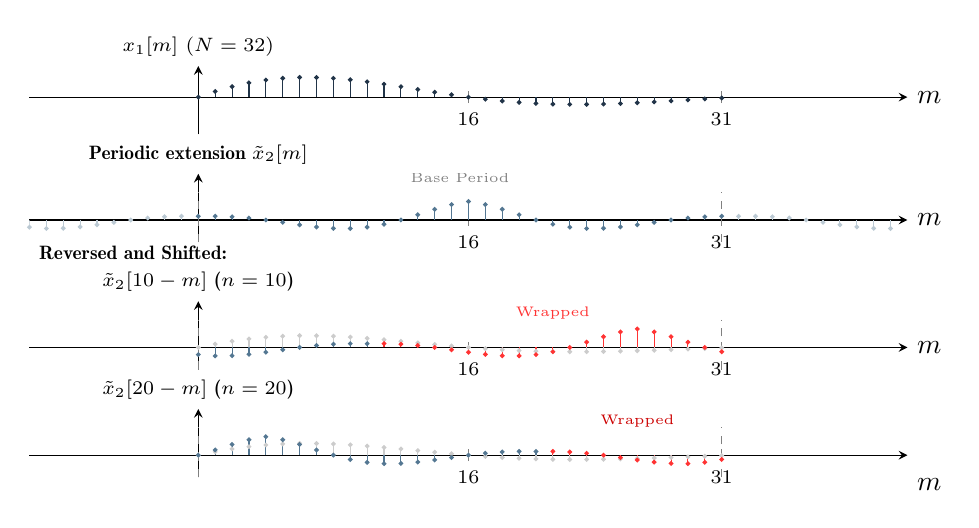
\begin{tikzpicture}
                    \node[font=\bfseries\scriptsize, anchor=west] at (0, -1.5) {Reversed and Shifted:};
                    \begin{axis}[
                        name=plot1,
                        width=1.05\textwidth, height=2.45cm,
                        axis lines=middle,
                        xmin=-10, xmax=42, ymin=-1.2, ymax=1.0,
                        xtick={0, 16, 31}, ytick=\empty,
                        xticklabel style={font=\scriptsize},
                        xlabel={$m$}, xlabel style={anchor=west},
                        ylabel={$x_1[m]$ ($N=32$)},
                        ylabel style={font=\scriptsize,anchor=south}
                        ]
                        \addplot[ycomb, PrimaryColor, mark=*, mark size=0.65pt, domain=0:31, samples=32] {sin(deg(x*pi/16)) * exp(-x/16)};
                    \end{axis}

                    \begin{axis}[
                        name=plot2,
                        at={(plot1.south)}, anchor=north, yshift=-0.5cm,
                        width=1.05\textwidth, height=2.45cm,
                        axis lines=middle,
                        xmin=-10, xmax=42, ymin=-1.2, ymax=2.5,
                        xtick={0, 16, 31}, ytick=\empty,
                        xticklabel style={font=\scriptsize},
                        xlabel={$m$}, x label style={anchor=west},
                        ylabel={Periodic extension $\tilde{x}_2[m]$},
                        ylabel style={font=\scriptsize\bfseries,anchor=south}
                        ]
                        \addplot[ycomb, SecondaryColor, mark=*, mark size=0.65pt, domain=0:31, samples=32] {cos(deg(x*pi/8)) * exp(-abs(x-16)/10)};
                        \addplot[ycomb, SecondaryColor!40, mark=*, mark size=0.65pt, domain=-10:-1, samples=10] {cos(deg((x+32)*pi/8)) * exp(-abs((x+32)-16)/10)};
                        \addplot[ycomb, SecondaryColor!40, mark=*, mark size=0.65pt, domain=32:41, samples=10] {cos(deg((x-32)*pi/8)) * exp(-abs((x-32)-16)/10)};
                        \draw[dashed, gray] (axis cs:0, -1.2) -- (axis cs:0, 1.5);
                        \draw[dashed, gray] (axis cs:31, -1.2) -- (axis cs:31, 1.5);
                        \node[font=\tiny, gray, anchor=south] at (axis cs:15.5, 1.5) {Base Period};
                    \end{axis}
                    \begin{axis}[
                        name=plot3,
                        at={(plot2.south)}, anchor=north, yshift=-0.75cm,
                        width=1.05\textwidth, height=2.45cm,
                        axis lines=middle,
                        xmin=-10, xmax=42, ymin=-1.2, ymax=2.5,
                        xtick={0, 16, 31}, ytick=\empty,
                        xticklabel style={font=\scriptsize},
                        xlabel={$m$}, x label style={anchor=west},
                        ylabel={$\tilde{x}_2[10-m]$ ($n=10$)},
                        ylabel style={font=\scriptsize\bfseries,anchor=south}
                        ]

                        \addplot[ycomb, gray!40, mark=*, mark size=0.65pt, domain=0:31, samples=32] {sin(deg(x*pi/16)) * exp(-x/16)};
                        \addplot[ycomb, SecondaryColor, mark=*, mark size=0.65pt, domain=0:10, samples=11] {cos(deg((10-x)*pi/8)) * exp(-abs((10-x)-16)/10)};
                        \addplot[ycomb, red!80, mark=*, mark size=0.65pt, domain=11:31, samples=21] {cos(deg((42-x)*pi/8)) * exp(-abs((42-x)-16)/10)};
                        \draw[dashed, gray] (axis cs:0, -1.2) -- (axis cs:0, 1.5);
                        \draw[dashed, gray] (axis cs:31, -1.2) -- (axis cs:31, 1.5);
                        \node[font=\tiny, red!80, anchor=south] at (axis cs:21, 1) {Wrapped};
                    \end{axis}

                    \begin{axis}[
                        name=plot4,
                        at={(plot3.south)}, anchor=north, yshift=-0.5cm,
                        width=1.05\textwidth, height=2.45cm,
                        axis lines=middle,
                        xmin=-10, xmax=42, ymin=-1.2, ymax=2.5,
                        xtick={0, 16, 31}, ytick=\empty,
                        xticklabel style={font=\scriptsize},
                        xlabel={$m$}, x label style={at={(1,-0.1)}, anchor=west},
                        ylabel={$\tilde{x}_2[20-m]$ ($n=20$)},
                        ylabel style={font=\scriptsize\bfseries,anchor=south}
                        ]
                        \addplot[ycomb, gray!40, mark=*, mark size=0.65pt, domain=0:31, samples=32] {sin(deg(x*pi/16)) * exp(-x/16)};
                        \addplot[ycomb, SecondaryColor, mark=*, mark size=0.65pt, domain=0:20, samples=21] {cos(deg((20-x)*pi/8)) * exp(-abs((20-x)-16)/10)};
                        \addplot[ycomb, red!80, mark=*, mark size=0.65pt, domain=21:31, samples=11] {cos(deg((52-x)*pi/8)) * exp(-abs((52-x)-16)/10)};
                        \draw[dashed, gray] (axis cs:0, -1.2) -- (axis cs:0, 1.5);
                        \draw[dashed, gray] (axis cs:31, -1.2) -- (axis cs:31, 1.5);
                        \node[font=\tiny, red!80!black, anchor=south] at (axis cs:26, 1) {Wrapped};
                    \end{axis}
                \end{tikzpicture}
            }
        \end{column}
    \end{columns}
\end{frame}

\begin{frame}{Linear Convolution via Zero-Padding}
    \begin{itemize}
        \item To use the FFT for standard \textbf{Linear Convolution} without introducing wrap-around artifacts from circularity, we must \textbf{zero-pad}!
        \item If $x_1[n]$ has length $L$ and $x_2[n]$ has length $M$, their linear convolution has length $\mathbf{L+M-1}$.
        \item We append zeros to both sequences until they share a length $N \ge L+M-1$. Now, applying circular convolution safely mirrors linear convolution because the wrap-around hits entirely zeros.
    \end{itemize}
    \vspace{0.4cm}
    \begin{algorithmbox}{Fast Convolution}
        \begin{enumerate}
            \item Choose $N \ge L+M-1$, ideally a power of 2 for maximum FFT performance.
            \item Zero-pad $x_1$ and $x_2$ to length $N$.
            \item Compute $X[1] = \text{FFT}(x_1, N)$ and $X[2] = \text{FFT}(x_2, N)$.
            \item Multiply Element-wise: $Y[k] = X[1][k] X[2][k]$.
            \item Compute $y[n] = \text{IFFT}(Y, N)$.
        \end{enumerate}
    \end{algorithmbox}
\end{frame}

\begin{frame}{Circular vs Linear Convolution: The Zero-Padding Fix}
    \begin{center}
        \resizebox{0.95\textwidth}{!}{
            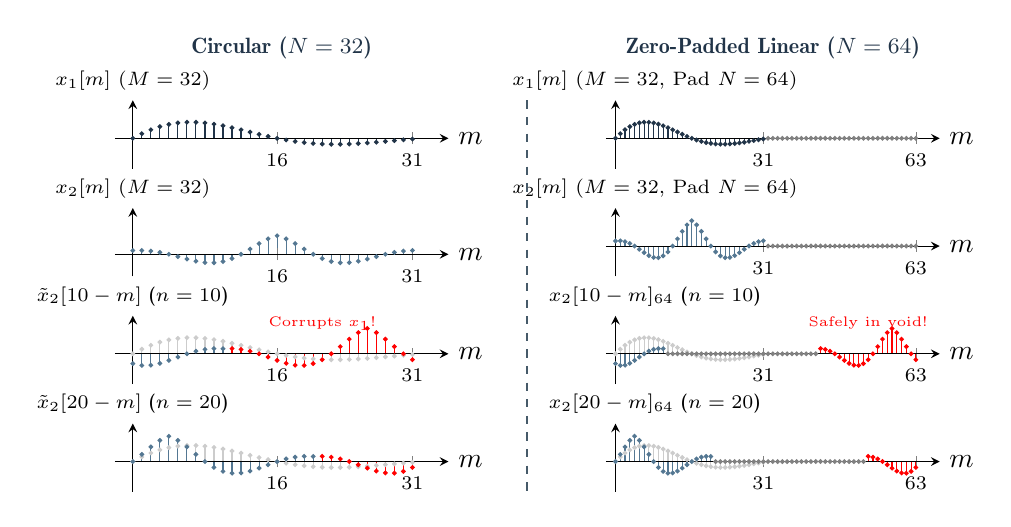
\begin{tikzpicture}
                % === LEFT: Insufficient padding ===
                \begin{axis}[
                    name=p0_L, width=0.48\textwidth, height=2.45cm,
                    ymin=-1.2, ymax=1.5, xmin=-2, xmax=35,
                    axis lines=middle, axis on top, xtick={0, 16, 31}, ytick=\empty,
                    xticklabel style={font=\scriptsize},
                    xlabel={$m$}, xlabel style={anchor=west},
                    ylabel={$x_1[m]$ ($M=32$)},
                    ylabel style={font=\scriptsize,anchor=south}
                    ]
                    \addplot[ycomb, PrimaryColor, mark=*, mark size=0.65pt, domain=0:31, samples=32] {sin(deg(x*pi/16)) * exp(-x/16)};
                \end{axis}

                \begin{axis}[
                    name=p1_L, at={(p0_L.south)}, anchor=north, yshift=-0.5cm,
                    width=0.48\textwidth, height=2.45cm,
                    ymin=-1.2, ymax=2.5, xmin=-2, xmax=35,
                    axis lines=middle, axis on top, xtick={0, 16, 31}, ytick=\empty,
                    xticklabel style={font=\scriptsize},
                    xlabel={$m$}, xlabel style={anchor=west},
                    ylabel={$x_2[m]$ ($M=32$)},
                    ylabel style={font=\scriptsize,anchor=south}
                    ]
                    \addplot[ycomb, SecondaryColor, mark=*, mark size=0.65pt, domain=0:31, samples=32] {cos(deg(x*pi/8)) * exp(-abs(x-16)/10)};
                \end{axis}

                \begin{axis}[
                    name=p2_L, at={(p1_L.south)}, anchor=north, yshift=-0.5cm,
                    width=0.48\textwidth, height=2.45cm,
                    ymin=-1.2, ymax=1.5, xmin=-2, xmax=35,
                    axis lines=middle, axis on top, xtick={0, 16, 31}, ytick=\empty,
                    xticklabel style={font=\scriptsize},
                    xlabel={$m$}, xlabel style={anchor=west},
                    ylabel={$\tilde{x}_2[10-m]$ ($n=10$)},
                    ylabel style={font=\scriptsize\bfseries,anchor=south}
                    ]
                    \addplot[ycomb, gray!40, mark=*, mark size=0.65pt, domain=0:31, samples=32] {sin(deg(x*pi/16)) * exp(-x/16)};
                    \addplot[ycomb, SecondaryColor, mark=*, mark size=0.65pt, domain=0:10, samples=11] {cos(deg((10-x)*pi/8)) * exp(-abs((10-x)-16)/10)};
                    \addplot[ycomb, red, mark=*, mark size=0.65pt, domain=11:31, samples=21] {cos(deg((42-x)*pi/8)) * exp(-abs((42-x)-16)/10)};
                    \node[font=\tiny, red] at (axis cs: 21, 1.2) {Corrupts $x_1$!};
                \end{axis}

                \begin{axis}[
                    name=p3_L, at={(p2_L.south)}, anchor=north, yshift=-0.5cm,
                    width=0.48\textwidth, height=2.45cm,
                    ymin=-1.2, ymax=1.5, xmin=-2, xmax=35,
                    axis lines=middle, axis on top, xtick={0, 16, 31}, ytick=\empty,
                    xticklabel style={font=\scriptsize},
                    xlabel={$m$}, xlabel style={anchor=west},
                    ylabel={$\tilde{x}_2[20-m]$ ($n=20$)},
                    ylabel style={font=\scriptsize\bfseries,anchor=south}
                    ]
                    \addplot[ycomb, gray!40, mark=*, mark size=0.65pt, domain=0:31, samples=32] {sin(deg(x*pi/16)) * exp(-x/16)};
                    \addplot[ycomb, SecondaryColor, mark=*, mark size=0.65pt, domain=0:20, samples=21] {cos(deg((20-x)*pi/8)) * exp(-abs((20-x)-16)/10)};
                    \addplot[ycomb, red, mark=*, mark size=0.65pt, domain=21:31, samples=11] {cos(deg((52-x)*pi/8)) * exp(-abs((52-x)-16)/10)};
                \end{axis}

                % === RIGHT: Sufficient padding ===
                \begin{axis}[
                    name=p0_R, at={(p0_L.east)}, anchor=west, xshift=2.0cm,
                    width=0.48\textwidth, height=2.45cm,
                    ymin=-1.2, ymax=1.5, xmin=-2, xmax=68,
                    axis lines=middle, axis on top, xtick={0, 31, 63}, ytick=\empty,
                    xticklabel style={font=\scriptsize},
                    xlabel={$m$}, xlabel style={anchor=west},
                    ylabel={$x_1[m]$ ($M=32$, Pad $N=64$)},
                    ylabel style={font=\scriptsize,anchor=south,xshift=0.5cm}
                    ]
                    \addplot[ycomb, PrimaryColor, mark=*, mark size=0.65pt, domain=0:31, samples=32] {sin(deg(x*pi/16)) * exp(-x/16)};
                    \addplot[ycomb, gray, mark=*, mark size=0.65pt, domain=32:63, samples=32] {0};
                \end{axis}

                \begin{axis}[
                    name=p1_R, at={(p0_R.south)}, anchor=north, yshift=-0.5cm,
                    width=0.48\textwidth, height=2.45cm,
                    ymin=-1.2, ymax=1.5, xmin=-2, xmax=68,
                    axis lines=middle, axis on top, xtick={0, 31, 63}, ytick=\empty,
                    xticklabel style={font=\scriptsize},
                    xlabel={$m$}, xlabel style={anchor=west},
                    ylabel={$x_2[m]$ ($M=32$, Pad $N=64$)},
                    ylabel style={font=\scriptsize,anchor=south,xshift=0.5cm}
                    ]
                    \addplot[ycomb, SecondaryColor, mark=*, mark size=0.65pt, domain=0:31, samples=32] {cos(deg(x*pi/8)) * exp(-abs(x-16)/10)};
                    \addplot[ycomb, gray, mark=*, mark size=0.65pt, domain=32:63, samples=32] {0};
                \end{axis}

                \begin{axis}[
                    name=p2_R, at={(p1_R.south)}, anchor=north, yshift=-0.5cm,
                    width=0.48\textwidth, height=2.45cm,
                    ymin=-1.2, ymax=1.5, xmin=-2, xmax=68,
                    axis lines=middle, axis on top, xtick={0, 31, 63}, ytick=\empty,
                    xticklabel style={font=\scriptsize},
                    xlabel={$m$}, xlabel style={anchor=west},
                    ylabel={$x_2[10-m]_{64}$ ($n=10$)},
                    ylabel style={font=\scriptsize\bfseries,anchor=south,xshift=0.5cm}
                    ]
                    \addplot[ycomb, gray!40, mark=*, mark size=0.65pt, domain=0:31, samples=32] {sin(deg(x*pi/16)) * exp(-x/16)};
                    \addplot[ycomb, SecondaryColor, mark=*, mark size=0.65pt, domain=0:10, samples=11] {cos(deg((10-x)*pi/8)) * exp(-abs((10-x)-16)/10)};
                    \addplot[ycomb, gray, mark=*, mark size=0.65pt, domain=11:42, samples=32] {0};
                    \addplot[ycomb, red, mark=*, mark size=0.65pt, domain=43:63, samples=21] {cos(deg((74-x)*pi/8)) * exp(-abs((74-x)-16)/10)};
                    \node[font=\tiny, red] at (axis cs: 53, 1.2) {Safely in void!};
                \end{axis}

                \begin{axis}[
                    name=p3_R, at={(p2_R.south)}, anchor=north, yshift=-0.5cm,
                    width=0.48\textwidth, height=2.45cm,
                    ymin=-1.2, ymax=1.5, xmin=-2, xmax=68,
                    axis lines=middle, axis on top, xtick={0, 31, 63}, ytick=\empty,
                    xticklabel style={font=\scriptsize},
                    xlabel={$m$}, xlabel style={anchor=west},
                    ylabel={$x_2[20-m]_{64}$ ($n=20$)},
                    ylabel style={font=\scriptsize\bfseries,anchor=south,xshift=0.5cm}
                    ]
                    \addplot[ycomb, gray!40, mark=*, mark size=0.65pt, domain=0:31, samples=32] {sin(deg(x*pi/16)) * exp(-x/16)};
                    \addplot[ycomb, SecondaryColor, mark=*, mark size=0.65pt, domain=0:20, samples=21] {cos(deg((20-x)*pi/8)) * exp(-abs((20-x)-16)/10)};
                    \addplot[ycomb, gray, mark=*, mark size=0.65pt, domain=21:52, samples=32] {0};
                    \addplot[ycomb, red, mark=*, mark size=0.65pt, domain=53:63, samples=11] {cos(deg((84-x)*pi/8)) * exp(-abs((84-x)-16)/10)};
                \end{axis}

                % Titles
                \node[font=\footnotesize\bfseries, PrimaryColor, anchor=south] at ([yshift=0.4cm]p0_L.north) {Circular ($N = 32$)};
                \node[font=\footnotesize\bfseries, PrimaryColor, anchor=south] at ([yshift=0.4cm]p0_R.north) {Zero-Padded Linear ($N = 64$)};

                % Divider
                \draw[dashed, DarkGray, thick] ($(p0_L.north east)!0.5!(p0_R.north west)$) -- ($(p3_L.south east)!0.5!(p3_R.south west)$);
            \end{tikzpicture}
        }
    \end{center}
    \vspace{-0.2cm}
    \begin{itemize}
        \item \textbf{Left:} $N=32 < L+M-1=63$ — convolution tail wraps around, corrupting early $x_1$ samples!
        \item \textbf{Right:} $N=64 \ge 63$ — wrapped tail comfortably hits the padding void ($x_1=0$). Circular $=$ Linear!
    \end{itemize}
\end{frame}

\begin{frame}{Fast Convolution Complexity Analysis}
    \begin{itemize}
        \item How much faster is this really?
        \item \textbf{Direct Linear Convolution:} Takes $O(L \cdot M)$ operations.
              If $L \approx M \approx N/2$, naive convolution takes roughly $\mathbf{O(N^2)}$ steps.
        \item \textbf{Fast Convolution (using Radix-2 FFT):}
              \begin{itemize}
                  \item 2 Forward FFTs: $2 \times O(N \log N)$
                  \item 1 Element-wise multiplication: $O(N)$
                  \item 1 Inverse FFT: $O(N \log N)$
              \end{itemize}
              Total time: $\mathbf{O(N \log N)}$ complex multiplications.
    \end{itemize}
    \begin{insightbox}{Real-world magnitude}
        Applying a 1-second reverb filter ($L = 44,100$) to 1-second of audio ($M = 44,100$):
        \begin{itemize}
            \item \textbf{Naive:} $L \times M \approx 1.94 \times 10^9$ operations.
            \item \textbf{Fast Convolution:} Padding to $N = 131,072 = 2^{17}$, taking $3 \times (N \log_2 N) \approx 6.6 \times 10^6$ operations.
            \item A massive speedup of purely algorithmic origin allowing real-time high-fidelity audio processing.
        \end{itemize}
    \end{insightbox}
\end{frame}

\section{FFT for Prime Lengths}

\begin{frame}{What if $N$ is Prime? Bluestein's Algorithm}
    \begin{itemize}
        \item We know Cooley-Tukey yields $O(N \log N)$ performance for powers of 2 (or composite $N = N_1 N_2$). But what if $N$ is a large prime number (e.g., $N = 1,000,003$)?
        \item Then $N_1=1$, and Cooley-Tukey devolves right back to $O(N^2)$.
        \item \textbf{Bluestein's Algorithm} bounds any DFT constraint to $O(N \log N)$ by cleverly expressing the DFT as a linear convolution!
    \end{itemize}
    \vspace{0.3cm}
    \begin{insightbox}{The Chirp-Z Identity}
        Start with the algebraic identity for powers:
        \begin{equation*}
            (k-n)^2 = k^2 - 2kn + n^2 \implies kn = -\frac{(k-n)^2}{2} + \frac{k^2}{2} + \frac{n^2}{2}
        \end{equation*}
        Using this, we can substitute $kn$ in the twiddle factor $W_N^{kn} = W_{2N}^{2kn}$ giving:
        \begin{equation*}
            W_N^{kn} = W_{2N}^{-(k-n)^2} W_{2N}^{k^2} W_{2N}^{n^2}
        \end{equation*}
    \end{insightbox}
\end{frame}

\begin{frame}{Bluestein's Algorithm Derivation}
    \begin{itemize}
        \item Applying the Chirp-Z Identity to the DFT definition:
              \begin{align*}
                  X[k] & = \sum_{n=0}^{N-1} x[n] W_N^{kn}                                                                                           \\
                       & = \sum_{n=0}^{N-1} x[n] \left(W_{2N}^{-(k-n)^2} W_{2N}^{k^2} W_{2N}^{n^2}\right)                                           \\
                       & = W_{2N}^{k^2} \sum_{n=0}^{N-1} \underbrace{\left(x[n] W_{2N}^{n^2}\right)}_{a[n]} \underbrace{W_{2N}^{-(k-n)^2}}_{b[k-n]}
              \end{align*}
        \item The summation is precisely a \textbf{linear convolution} evaluated at index $k$!
              \begin{equation*}
                  X[k] = W_{2N}^{k^2} \cdot (a * b)[k]
              \end{equation*}
              where $a[n] = x[n] W_{2N}^{n^2}$ for $n \in [0, N-1]$ and the chirp filter $b[n] = W_{2N}^{-n^2}$ for $n \in [-(N-1), N-1]$.
        \item We can evaluate this convolution using fast convolution!
        \item But in this case we need to handle the padding of $b[n]$ with care as $n$ can be negative.
    \end{itemize}
\end{frame}

\begin{frame}{Visualizing Zero-Padding for Bluestein's Algorithm}
    \begin{center}
        \resizebox{0.95\textwidth}{!}{
            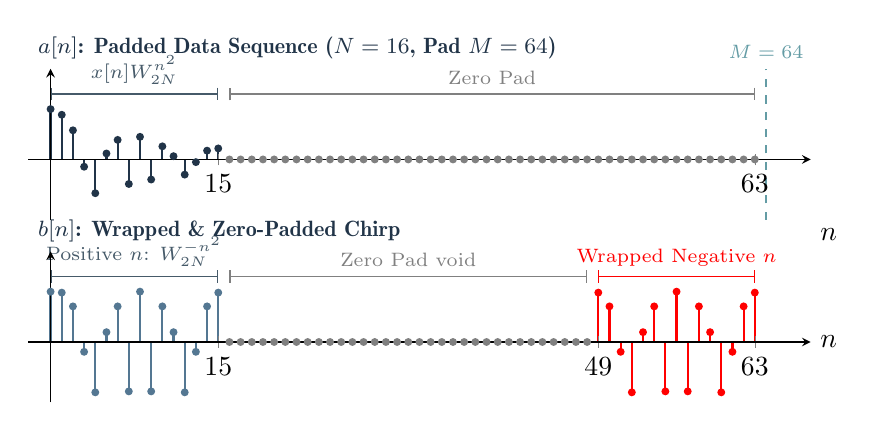
\begin{tikzpicture}
                \begin{axis}[
                        name=plotA, width=0.95\textwidth, height=3.5cm,
                        ymin=-1.2, ymax=1.8, xmin=-2, xmax=68,
                        axis lines=middle, axis on top, xtick={0, 15, 63}, ytick=\empty,
                        xlabel={$n$}, x label style={at={(1,-0.1)}, anchor=west},
                        clip=false
                    ]
                    \addplot[ycomb, PrimaryColor, thick, mark=*, mark size=1.0pt, domain=0:15, samples=16] {cos(deg(x*x*pi/16)) * exp(-x/10)};
                    \addplot[ycomb, gray, thick, mark=*, mark size=1.0pt, domain=16:63, samples=48] {0};

                    \draw[|-|, DarkGray] (axis cs:0, 1.3) -- (axis cs:15, 1.3) node[midway, above, font=\scriptsize] {$x[n]W_{2N}^{n^2}$};
                    \draw[|-|, gray] (axis cs:16, 1.3) -- (axis cs:63, 1.3) node[midway, above, font=\scriptsize] {Zero Pad};

                    \draw[dashed, AccentColor, thick] (axis cs: 64, -1.2) -- (axis cs: 64, 1.8) node[above, font=\scriptsize, align=center] {$M=64$};
                \end{axis}
                \node[font=\footnotesize\bfseries, PrimaryColor, anchor=south west] at (plotA.north west) {$a[n]$: Padded Data Sequence ($N=16$, Pad $M=64$)};

                \begin{axis}[
                        name=plotB, at={(plotA.south)}, anchor=north, yshift=-0.4cm,
                        width=0.95\textwidth, height=3.5cm,
                        ymin=-1.2, ymax=1.8, xmin=-2, xmax=68,
                        axis lines=middle, axis on top, xtick={0, 15, 49, 63}, ytick=\empty,
                        xlabel={$n$}, x label style={anchor=west},
                        clip=false
                    ]
                    \addplot[ycomb, SecondaryColor, thick, mark=*, mark size=1.0pt, domain=0:15, samples=16] {cos(deg(x*x*pi/16))};
                    \addplot[ycomb, gray, thick, mark=*, mark size=1.0pt, domain=16:48, samples=33] {0};
                    \addplot[ycomb, red, thick, mark=*, mark size=1.0pt, domain=49:63, samples=15] {cos(deg((x-64)*(x-64)*pi/16))};

                    \draw[|-|, DarkGray] (axis cs:0, 1.3) -- (axis cs:15, 1.3) node[midway, above, font=\scriptsize] {Positive $n$: $W_{2N}^{-n^2}$};
                    \draw[|-|, gray] (axis cs:16, 1.3) -- (axis cs:48, 1.3) node[midway, above, font=\scriptsize] {Zero Pad void};
                    \draw[|-|, red] (axis cs:49, 1.3) -- (axis cs:63, 1.3) node[midway, above, font=\scriptsize] {Wrapped Negative $n$};

                \end{axis}
                \node[font=\footnotesize\bfseries, PrimaryColor, anchor=south west] at (plotB.north west) {$b[n]$: Wrapped \& Zero-Padded Chirp};

            \end{tikzpicture}
        }
    \end{center}

    \vspace{-0.3cm}
    \begin{itemize}
        \item Linear convolution evaluates $b[k-n]$, so index ranges from $k-(N-1)$ to $k$.
        \item Note that $k-n$ can be negative, so we need to handle negative indices when they wrap around at $k - n \pmod{M}$.
        \item We allocate the \textbf{positive indices} of $b[n]$ at the start of the size-$M$ array, and the \textbf{negative indices} at the end, placing zeros in the middle to prevent overlapping.
        \item So, $M$ must be at least $2N-1$ to avoid overlapping.
    \end{itemize}
\end{frame}

\begin{frame}{Bluestein's Fast Convolution}
    \begin{itemize}
        \item How does solving a multiplication via convolution help?
        \item Because we can process linear convolution utilizing \textbf{Fast Convolution with Zero-Padding}!
        \item Sequence $a[n]$ has length $N$. Sequence $b[n]$ is evaluated for $n \in -(N-1) \dots (N-1)$, meaning its support length is $2N-1$.
        \item We can pick \textit{any} $M \ge 2N-1$ and zero-pad both sequences. We intentionally choose $M=2^m$ so we can use the highly efficient Radix-2 DIT FFT!
    \end{itemize}
    \vspace{0.4cm}
    \begin{algorithmbox}{Bluestein's FFT Algorithm}
        \begin{enumerate}
            \item Form sequence $a[n]$ and periodized $b[n]$ to size $M = 2^{\lceil \log_2(2N-1) \rceil}$.
            \item Compute $A = \text{FFT}(a, M)$ and $B = \text{FFT}(b, M)$ using Radix-2.
            \item Compute $Y[k] = A[k] B[k]$.
            \item Compute $y[n] = \text{IFFT}(Y, M)$.
            \item Multiply by $W_{2N}^{k^2}$: $X[k] = y[k] W_{2N}^{k^2}$ for $k=0 \dots N-1$.
        \end{enumerate}
    \end{algorithmbox}
\end{frame}

\end{document}
